\section{Revised results in alternative markets}
\label{sec:robustness}
SSE50 and the Nasdaq Composite provide comparisons under the same model families and residual ablation. Corrected SSE50 has train/validation/test counts of 1500/500/1919, whereas Nasdaq retains 2000/500/1554. SSE50 uses Chinese monthly EPU and Nasdaq uses US monthly EPU. Differences in markets and estimation lengths limit direct cross-market interpretation; neither sample is an untouched independent external validation set.

\subsection{Point losses}
\begin{table}[htbp]\centering
\caption{Calendar-corrected SSE50 point losses, $N=1919$.}
\label{tab:sse50_metrics}
\begin{tabular}{lrrr}\toprule Model & MSE & MAE & QLIKE\\\midrule
HAR & 4.826226 & 1.717026 & 3.872429\\
GARCH(1,1) & 7.537442 & 2.043060 & 1.586804\\
XGB-Market & 4.940740 & 1.740321 & 4.753901\\
XGB-AR & 4.954984 & 1.741490 & 4.697720\\
DEC & 4.972472 & 1.718639 & 3.672557\\\bottomrule
\end{tabular}
\end{table}
\begin{table}[htbp]\centering
\caption{Revised Nasdaq point losses, $N=1554$.}
\label{tab:nas_metrics}
\begin{tabular}{lrrr}\toprule Model & MSE & MAE & QLIKE\\\midrule
HAR & 5.292393 & 1.814872 & 3.994306\\
GARCH(1,1) & 7.110225 & 1.894212 & 1.498305\\
XGB-Market & 5.284620 & 1.767569 & 4.279836\\
XGB-AR & 5.302560 & 1.761263 & 4.224645\\
DEC & 5.369943 & 1.772158 & 3.895152\\\bottomrule
\end{tabular}
\end{table}

In SSE50, DEC improves QLIKE and MAE relative to both XGB comparators but worsens MSE. In Nasdaq, it improves QLIKE while worsening both MSE and MAE. Across all three markets, GARCH has the lowest QLIKE, followed by DEC. The gains associated with including EPU are therefore loss-dependent and do not imply general dominance.

\subsection{Why the Nasdaq specification changes}
The historical single-start 12-month Beta fit has training SSE approximately 1780.2771 on 299 residual pairs and validation MSE approximately 4.3325. Multistart estimation finds a lower training SSE of approximately 1779.2408, but its validation MSE increases to 5.0476. The 12-month exponential Almon candidate has validation MSE 4.3446 and is then selected among the six candidates. The switch follows the validation rule; it is not a choice based on favorable test QLIKE.

Fixing the historical 12-month Beta family while repairing only the solver produces Nasdaq test MSE 5.434646 and QLIKE 3.791512. Re-selecting by the stated validation rule produces MSE 5.369943 and QLIKE 3.895152. An inferior training optimum may have behaved like implicit regularization in this finite sample, but this is an explanatory hypothesis, not a reason to claim that the old optimizer correctly minimized its objective.

Archived DEC has MSE 5.423666 and QLIKE 3.794736. The selected revised Almon model therefore improves MSE by about 0.99\% while worsening QLIKE by about 2.65\%. Both changes must be reported. In SSE50, calendar correction and solver revision occur together, so the full difference from archived results cannot be attributed entirely to the optimizer. A separate calendar-control experiment is retained in Appendix~\ref{app:training}.

\subsection{Graphical comparisons}
The figures retain the same current-result images as the Chinese edition. Weight panels show the validation-stage selection, not invariant test-period coefficients. Both Chinese markets select 24-month exponential Almon weights; Nasdaq selects 12 months. Boundary solutions and re-estimation prevent a stable policy-transmission interpretation.

\begin{figure}[htbp]\centering
\begin{minipage}{.48\textwidth}\centering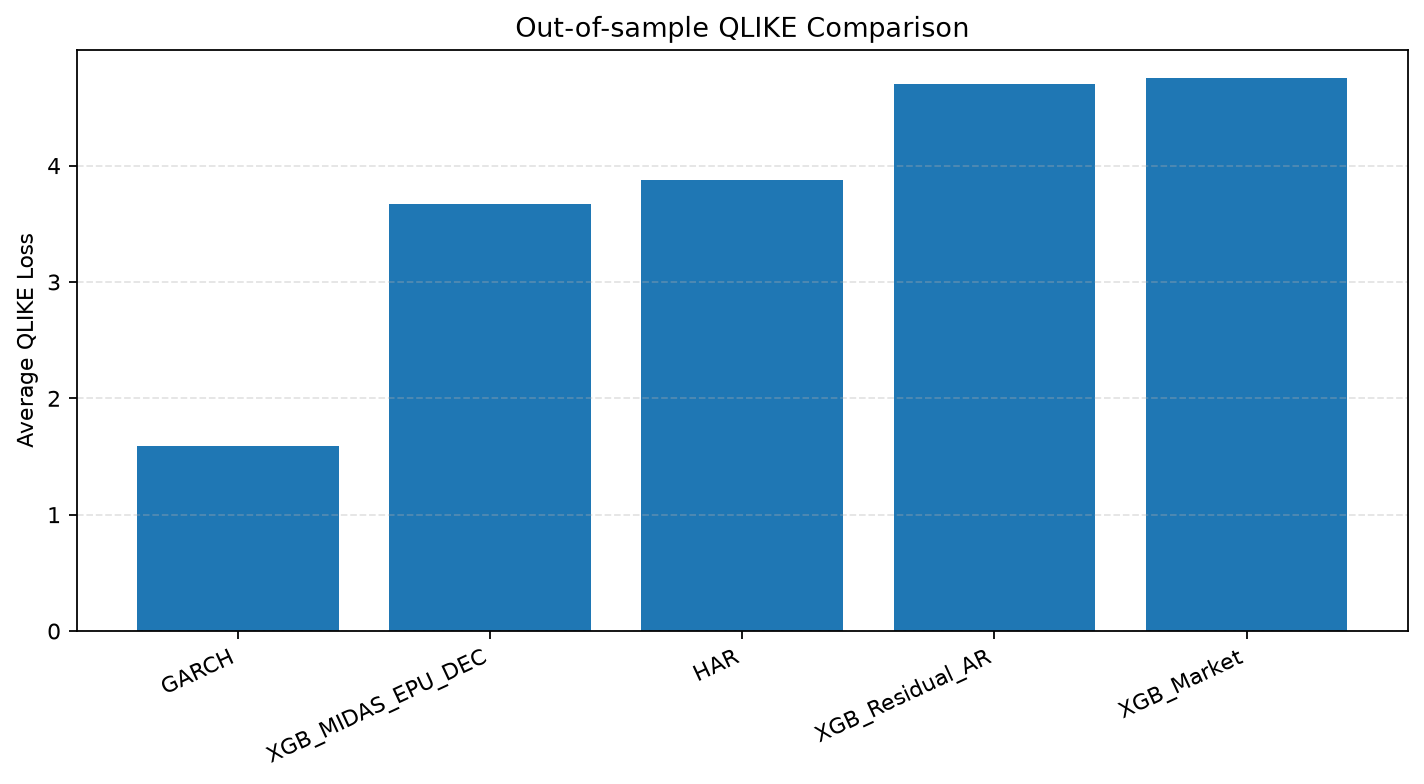
\includegraphics[width=\linewidth]{../../results/revised/sse50/fig_metrics_bar.png}\par{\small QLIKE}\end{minipage}\hfill
\begin{minipage}{.48\textwidth}\centering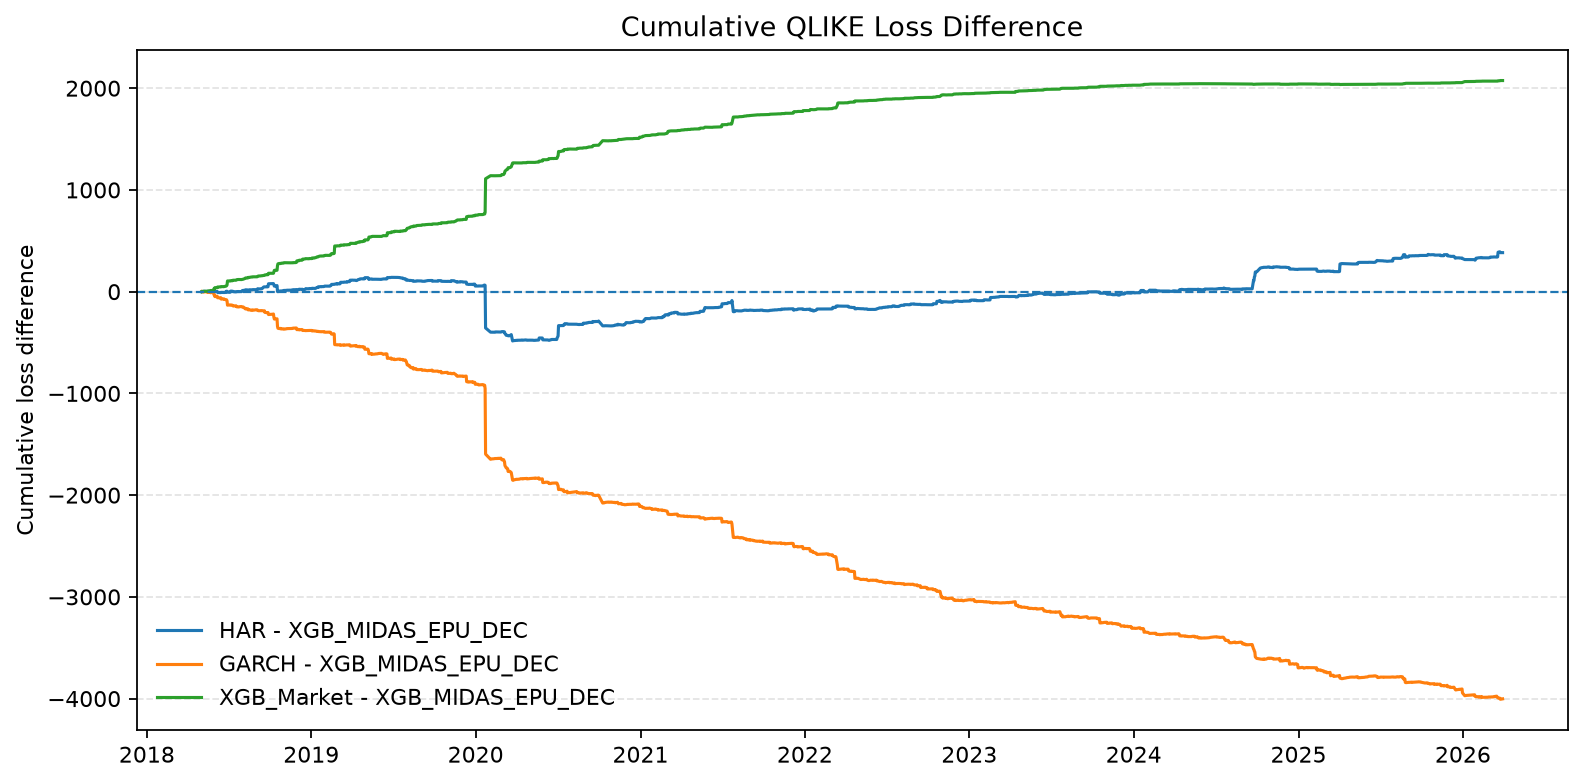
\includegraphics[width=\linewidth]{../../results/revised/sse50/fig_cumulative_qlike_diff.png}\par{\small Cumulative QLIKE differences}\end{minipage}\par\medskip
\begin{minipage}{.48\textwidth}\centering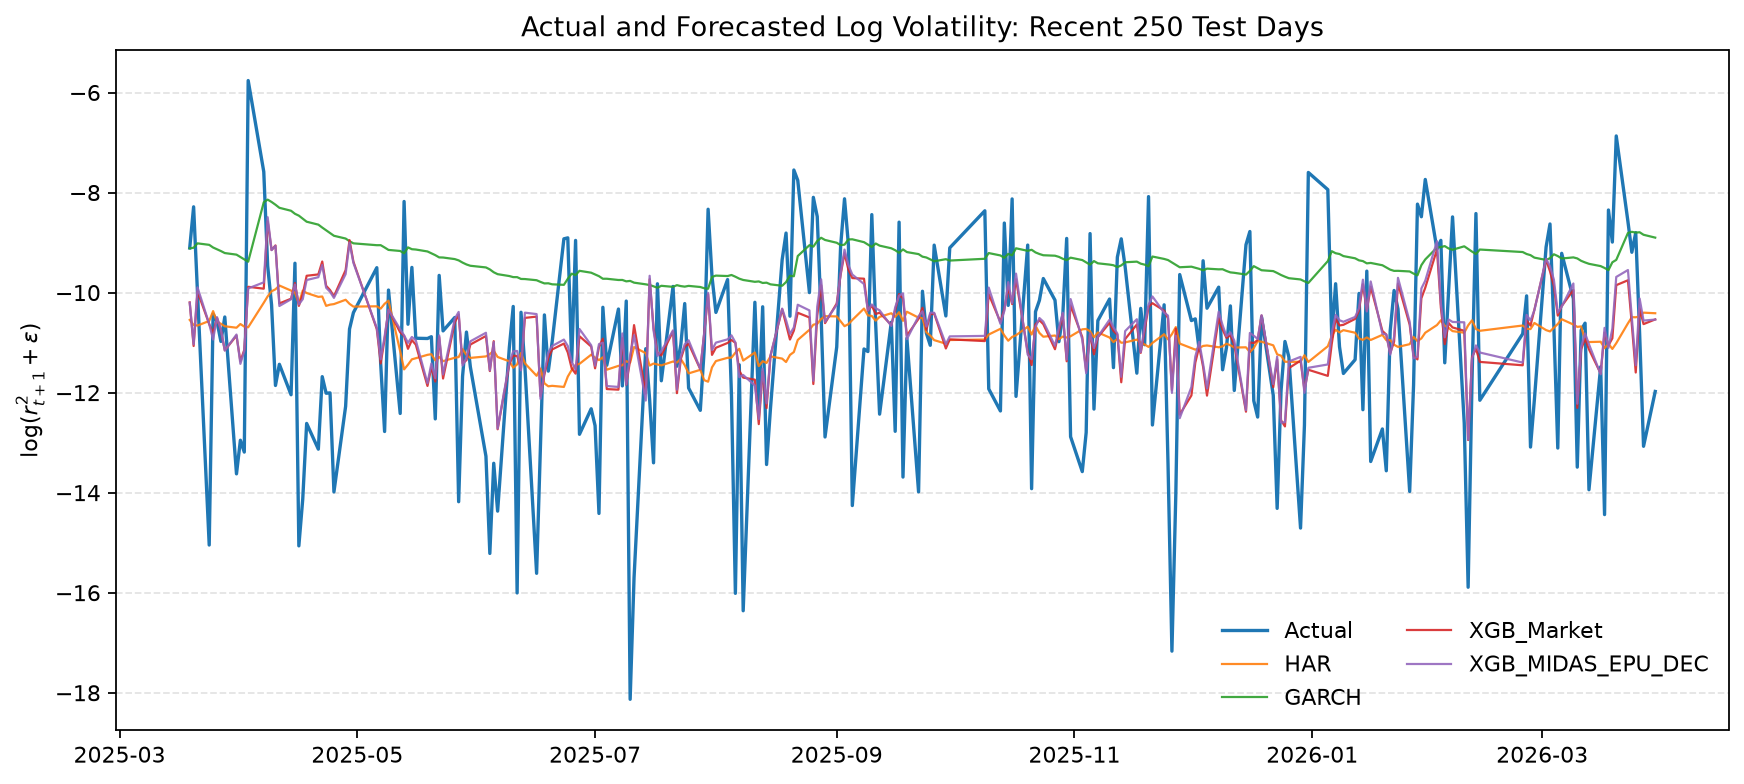
\includegraphics[width=\linewidth]{../../results/revised/sse50/fig_prediction_series_recent.png}\par{\small Recent predictions}\end{minipage}\hfill
\begin{minipage}{.48\textwidth}\centering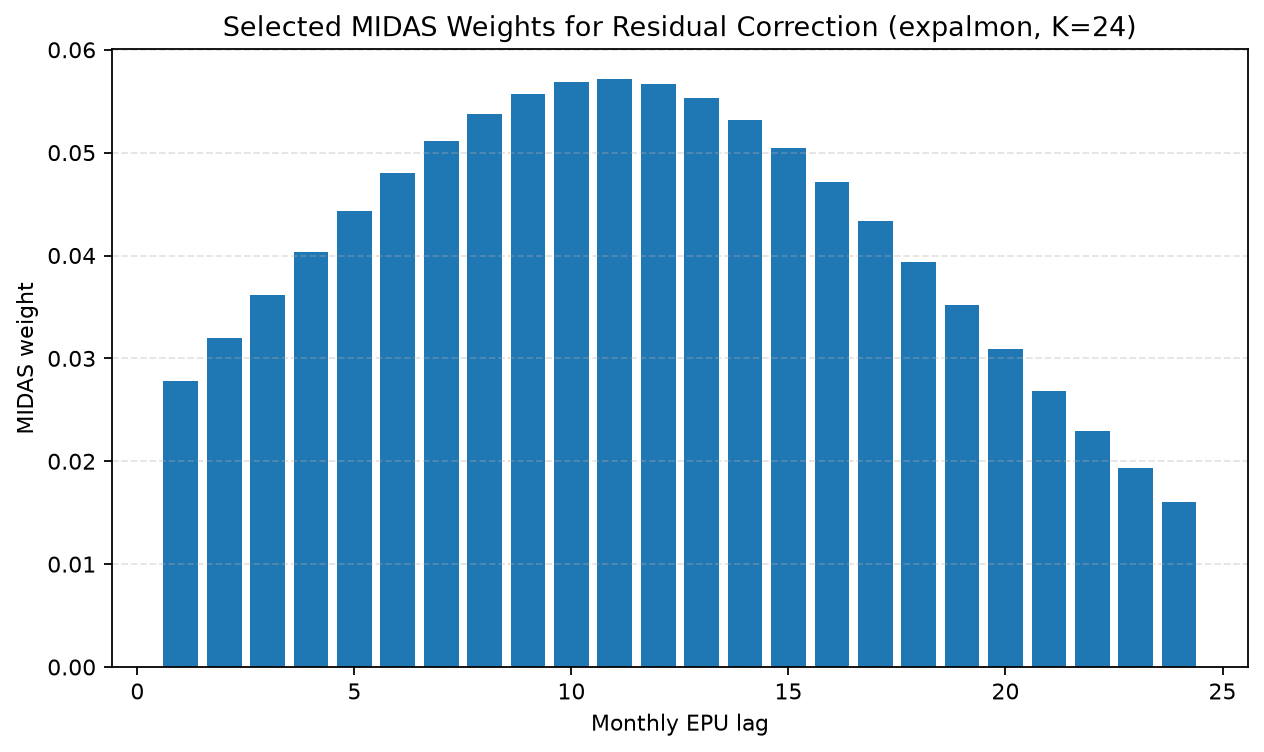
\includegraphics[width=\linewidth]{../../results/revised/sse50/fig_midas_weights.png}\par{\small Validation-selected weights}\end{minipage}
\caption{Revised SSE50 results after the confirmed holiday correction.}
\label{fig:sse50_robustness_panel}
\end{figure}
\begin{figure}[htbp]\centering
\begin{minipage}{.48\textwidth}\centering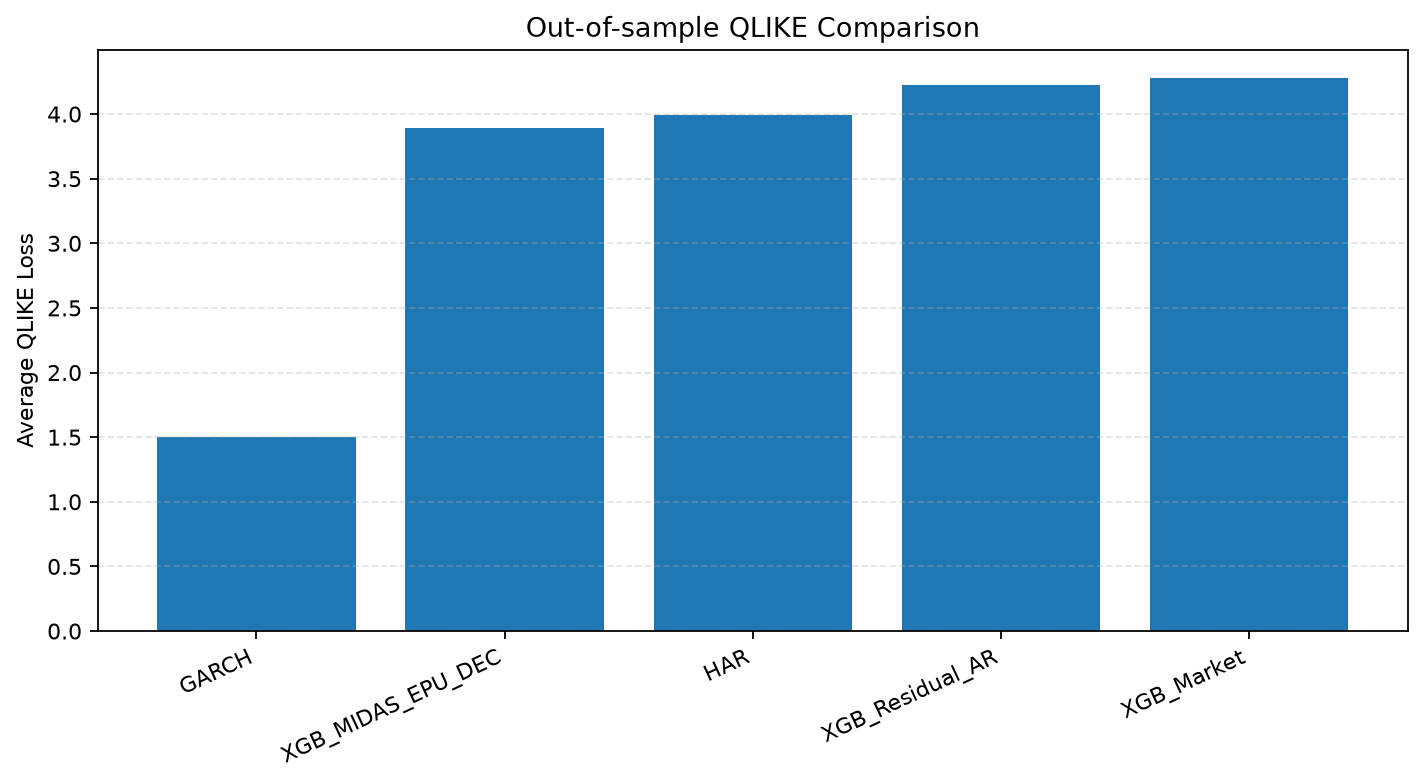
\includegraphics[width=\linewidth]{../../results/revised/nasdaq/fig_metrics_bar.png}\par{\small QLIKE}\end{minipage}\hfill
\begin{minipage}{.48\textwidth}\centering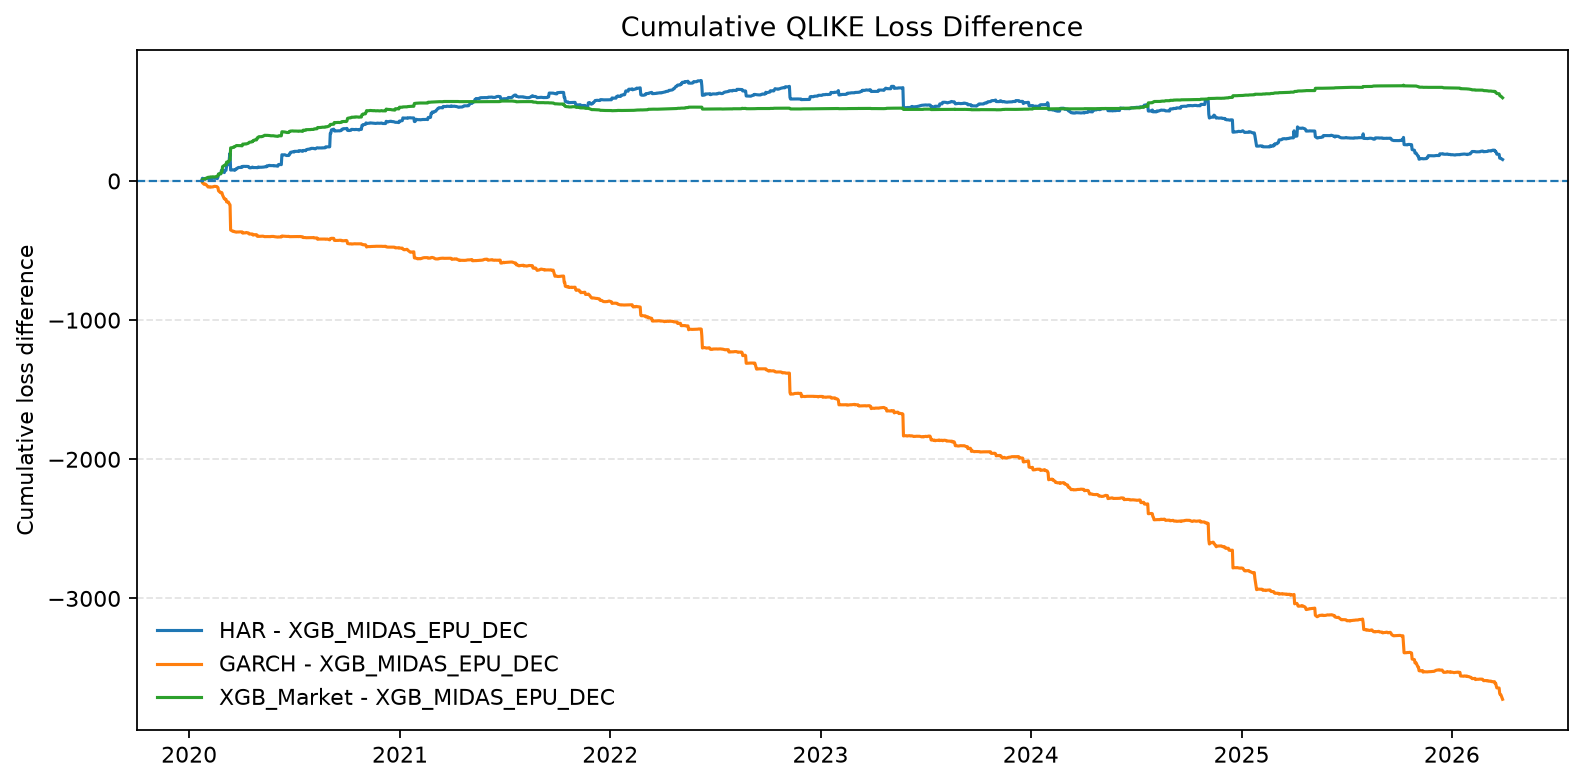
\includegraphics[width=\linewidth]{../../results/revised/nasdaq/fig_cumulative_qlike_diff.png}\par{\small Cumulative QLIKE differences}\end{minipage}\par\medskip
\begin{minipage}{.48\textwidth}\centering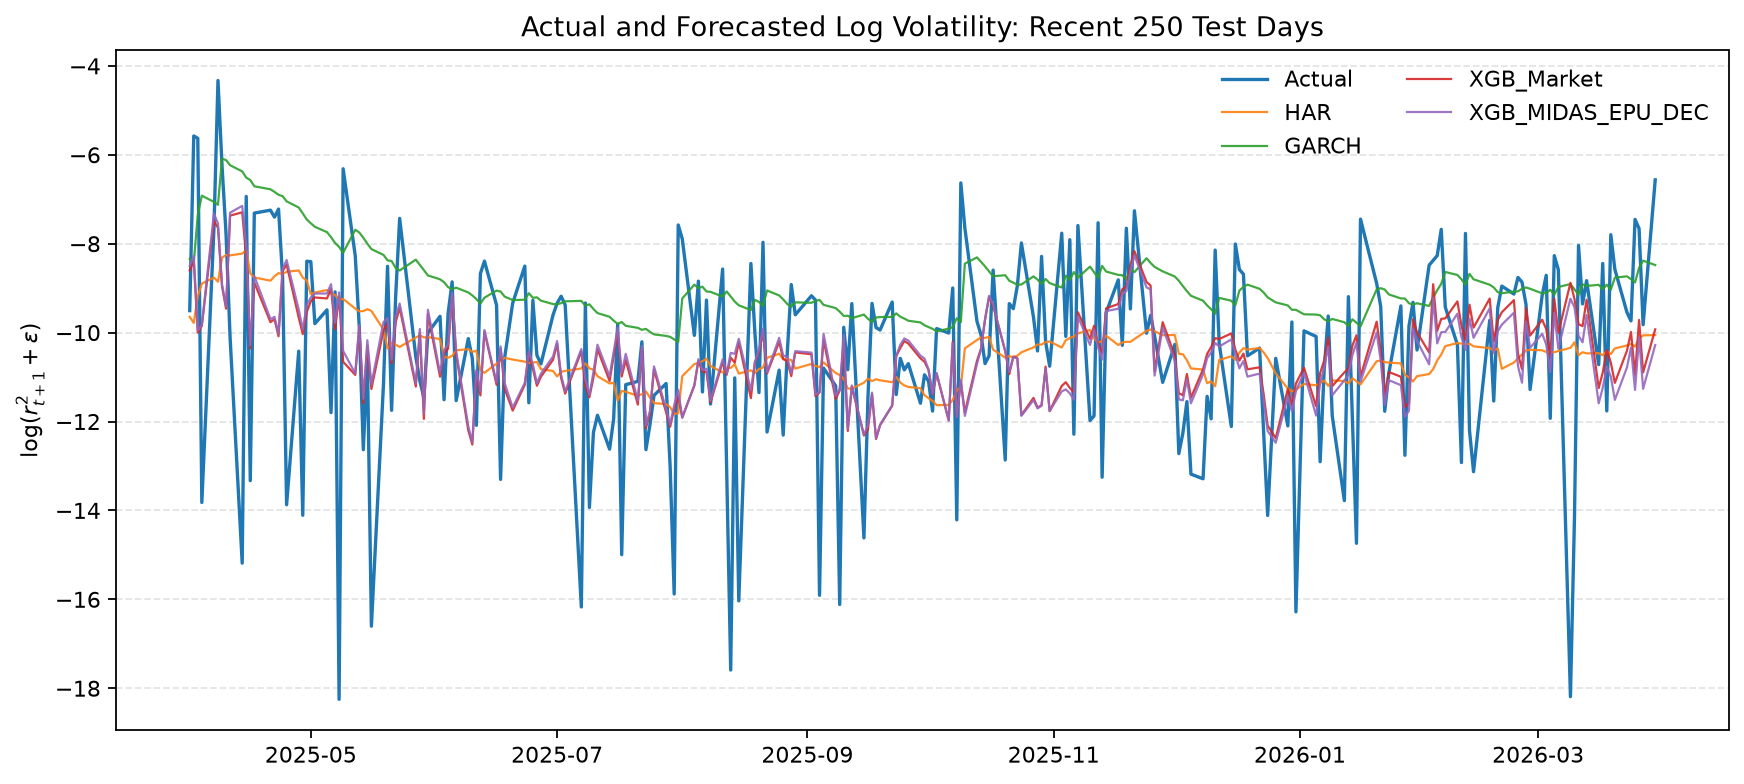
\includegraphics[width=\linewidth]{../../results/revised/nasdaq/fig_prediction_series_recent.png}\par{\small Recent predictions}\end{minipage}\hfill
\begin{minipage}{.48\textwidth}\centering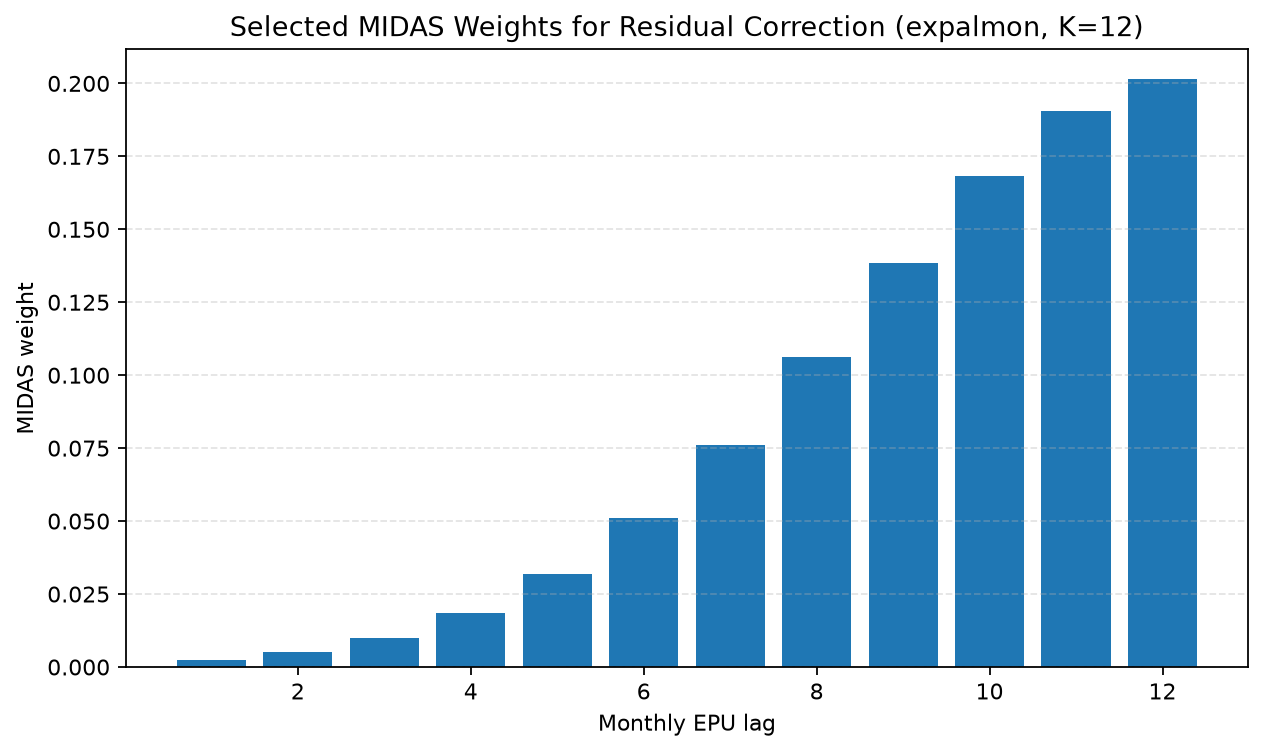
\includegraphics[width=\linewidth]{../../results/revised/nasdaq/fig_midas_weights.png}\par{\small Validation-selected weights}\end{minipage}
\caption{Revised Nasdaq results with the validation-selected Almon specification.}
\label{fig:nas_robustness_panel}
\end{figure}

\subsection{Ablation and scope of evidence}
Mean QLIKE advantages of DEC relative to XGB-AR are 1.168972, 1.025163, and 0.329494 for CSI300, SSE50, and Nasdaq. Holm-adjusted normal-reference $p$-values across the 18 comparisons are approximately $6.61\times10^{-12}$, $4.65\times10^{-7}$, and 0.0215. These are exploratory indications under the retrospective and selection constraints, not conclusive evidence of a population-wide advantage. DEC has higher MSE than XGB-AR in all three markets; the adjusted diagnostics do not support MSE improvement.

A useful next evaluation would lock the entire pipeline in advance, retain genuine release-time EPU vintages, and use a new time holdout. That design would test whether the observed loss-dependent pattern persists beyond the already examined samples.
\clearpage
